\section{Datenerfassung auf Intensivstationen}
\cite{marxIntensivmedizin2015c} verorten die Intensivmedizin im Spannungsfeld zwischen Heilen und Sterben. Eine Verlegung auf die Intensivstation erfolgt häufig infolge einer besonders schweren oder lebensbedrohlichen Erkrankung oder Verletzung. 
Ziel der Behandlung ist es, sofern möglich, den Patienten\footnote{Hier und im Rest der Arbeit umfasst das generische Maskulinum, sofern nicht anders angegeben, Personen beider Geschlechter.} so zu kurieren, dass diesem ein Weiterleben unabhängig von den besonderen technischen und personellen Möglichkeiten der Intensivmedizin möglich ist. Dafür wird eine besonders intensive Behandlung durch Ärzte und Pflegekräfte benötigt.

Technische Fortschritte und die Digitalisierung ermöglichen es, mehr Informationen über die Patienten zu erfassen und zu verarbeiten als je zuvor. Ärzte, Pflegekräfte, aber auch Angehörige werden so mit umfangreichen Mengen an Informationen konfrontiert. Dabei stellt die erfolgreiche Kommunikation zwischen Behandelnden eine wichtige Vorraussetzung für das Patientenoutcome dar. \cite{marxIntensivmedizin2015c} benennen Kommunikationsprobleme als wichtigen Faktor für erhöhte Krankenhausmortalitätsraten. Die Autoren beschreiben weiter, dass bis zu 50 \% der klinisch relevanten Informationen, die noch in der Morgenvisite zwischen Ärzten ausgetauscht wurden, schon in der Spätvisite des gleichen Tages nicht mehr übermittelt werden. %(Kap. 11.5.4)

Die Frage der effektiven Datenerfassung auf Intensivstationen ist somit eine über Leben und Tod. Dennoch kommt es aus unterschiedlichen Gründen vor, dass Informationen über den Gesundheitszustand der Patienten ungenau oder in zu geringem Umfang digital erfasst werden. 

Gegenstand der vorliegenden Arbeit ist der Versuch, mittels maschinellem Lernen einen Beitrag zur Lösung dieses Problems zu leisten.\footnote{Der komplette Programmcode der Modelle, Skripte zur Datenaufbereitung und mehr liegen in folgendem Git-Repository vor: \url{https://github.com/mahathu/bachelorarbeit}}

\subsection{medizinische Scores} \label{section:scores}

In \textit{Die Intensivmedizin} \citep{marxIntensivmedizin2015c} ist der Begriff des Scores folgendermaßen definiert:

\begin{itquote}
    "Ein Score ist der Versuch, eine komplexe klinische Situation auf einen eindimensionalen Punktwert abzubilden. Eine solche Reduktion verfolgt das Ziel, übergreifende Aspekte wie Schweregrad oder Prognose als Kombination einzelner Fakten objektiv zu fassen, um sie dann in unterschiedlichen Kollektiven vergleichend darstellen zu können."
\end{itquote}

Es handelt sich bei einem Score häufig um die Kombination mehrerer erfassbarer Werte, wie beispielsweise der Herzfrequenz oder der Reaktion auf bestimmte Reize. Auch allgemeine Informationen über den Patienten wie das Alter oder bekannte Vorerkrankungen können je nach Score berücksichtigt werden. Die Bestimmung eines Score-Werts stellt also den Versuch dar, die komplexe, individuelle Situation eines Patienten auf einen eindimensionalen, numerischen Wert zu reduzieren. Dabei gehen unweigerlich Informationen verloren. Gleichzeitig erlaubt es die Erfassung von derartigen standardisierten Scores aber, auf einen Blick wichtige Informationen über den Zustand des Patienten zu erfassen. Ferner wird durch eine solche Reduktion auf das Wesentliche ermöglicht, den Krankheitsverlauf eines Patienten über einen längeren Zeitraum zu analysieren, oder die Symptomatik mehrerer Patienten leichter miteinander zu vergleichen. Ein weiterer Vorteil ist dass, unter Voraussetzung der richtigen Anwendung, die Vergabe von Scores weitestgehend unabhängig von der subjektiven Einschätzung des Arztes oder der Pflegekraft erfolgt \citep{marxIntensivmedizin2015c}.
%Eine Ausnahme unter den in den Datensätzen erfassten Werte bildet der CAM-ICU (siehe Abschnitt \ref{section:vorliegende_daten}). Das Ergebnis fällt hierbei entweder positiv oder negativ aus und stellt damit keinen Score im eigentlichen Sinne dar. 
Die Frage, ob es sich bei der Vorhersage der im Rahmen dieser Arbeit behandelten Scores um ein Regressions- oder ein Klassifikationsproblem handelt, wird in Abschnitt \ref{section:regrvsclf} behandelt. 

\subsection{Ziel der Arbeit}
Das Ziel der vorliegenden Arbeit ist es, mit Hilfe von maschinellem Lernen ein statistisches Modell zu entwickeln, um anhand von Freitexten medizinische Scores möglichst akkurat vorherzusagen. Die Entwicklung eines solchen Modells ermöglicht es unter anderem, die tatsächlich eingetragenen Werte mit den Vorhersagen des Modells zu vergleichen, um daraus Rückschlüsse über die Qualität der Datenerfassung an der Charité zu treffen.

\section{Maschinelles Lernen}
Der Begriff Maschinelles Lernen kennzeichnet einen modernen Ansatz in der Forschung an künstlicher Intelligenz. Obgleich die Anfänge des maschinellen Lernens bereits mehrere Jahrzehnte zurückliegen \citep{samuelStudiesMachineLearning1959, nilsson1965learning}, hat es sich im Zeitalter von Big Data und besonders leistungsstarken Rechnern zu einem der Forschungsschwerpunkte der modernen angewandten Informatik entwickelt. Algorithmen aus dem Bereich des Maschinellen Lernens ermöglichen es, anhand von Eingabedaten Vorhersagen über Eigenschaften noch unbekannter Daten zu treffen \citep{mitchellMachineLearning1997}. Im gleichen Werk definiert der Autor diesen Prozess folgendermaßen:

\begin{itquote}
    {\foreignlanguage{english}{"A computer program is said to learn from experience E with respect to some class of tasks T and performance measure P, if its performance at tasks in T, as measured by P, improves with experience E."}}
\end{itquote}

"Lernen" bezeichnet hierbei die besondere Fähigkeit eines Computerprogramms, sich anhand neuer Eingabedaten selbstständig anzupassen und zu verbessern. Dies unterscheidet das maschinelle Lernen von herkömmlichen Verfahren der inferentiellen Statistik. Im Allgemeinen wird der Prozess des Lernens durch den Versuch modelliert, eine vorher festgelegte, wohldefinierte Verlustfunktion zu minimieren. % \reffig{fig:optimierung}
Die dafür existieren numerischen Optimierungsverfahren sind ein grundlegender Untersuchungsgegenstand in der Forschung am maschinellen Lernen.

Bei Regressionsproblemen stellt beispielsweise die mittlere absolute Abweichung (\textit{mean absolute error}) der Vorhersagen zu den tatsächlichen Werten eine solche Verlustfunktion dar, die es zu minimieren gilt. Abbildung \ref{fig:linear} zeigt einen Datensatz, dessen Werte einem annähernd linearen Verlauf folgen. Ihr Zusammenhang lässt sich also anhand einer Regressionsgerade $f(x) = mx + t$ (schwarze Linie) modellieren. Je nach Wahl der Parameter $m$ und $t$ ist die Funktionsgerade mehr oder weniger geeignet, die tatsächliche Verteilung der Werte zu beschreiben. Je besser die beiden Funktionsparameter gewählt werden, desto geringer sind die Residuen (rote Linien), und desto mehr nähert sich die Verlustfunktion ihrem Minimum an.

% \begin{figure}[htbp]
%     \captionsetup{justification=centering}

%     \centering
%     %\subfloat[$f(x,y) = \frac{x^2 - y^2}{5}$]{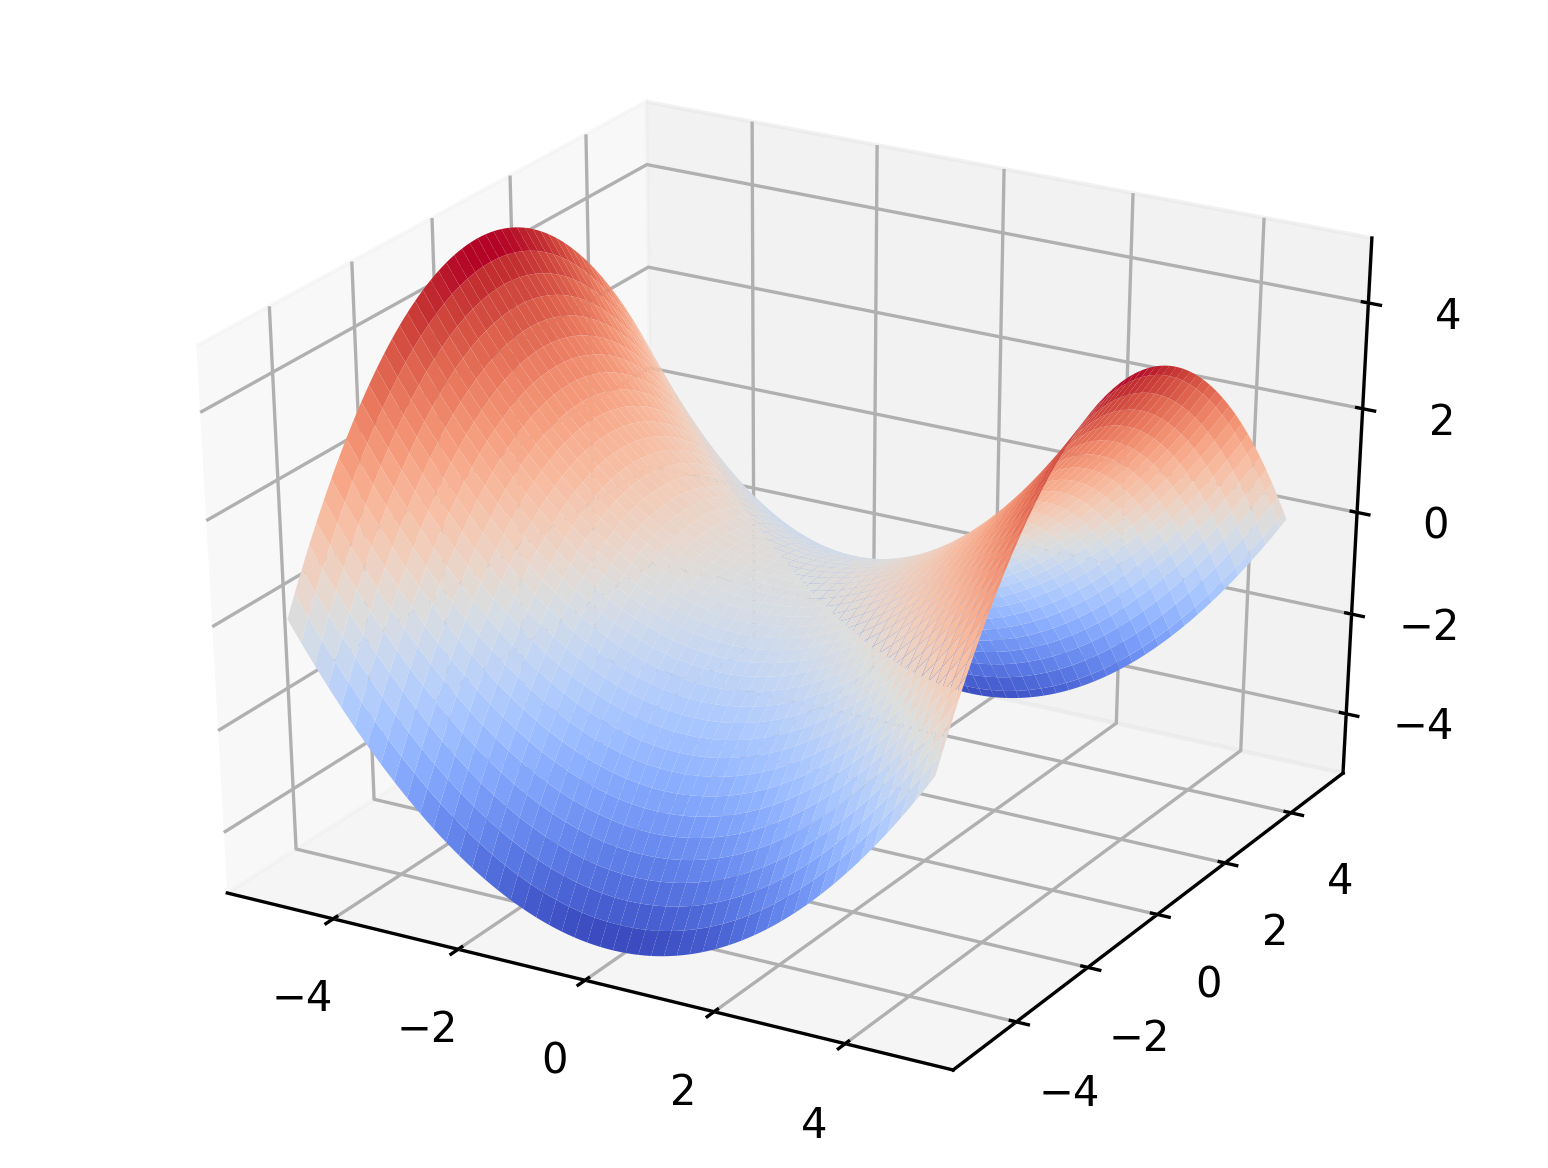
\includegraphics[width=0.48\textwidth]{3d_pringle}} 
%     \subfloat[$f(x,y) = \left(20-x\right)^\frac{5}{4}+10\left(x-y^2\right)^2$]{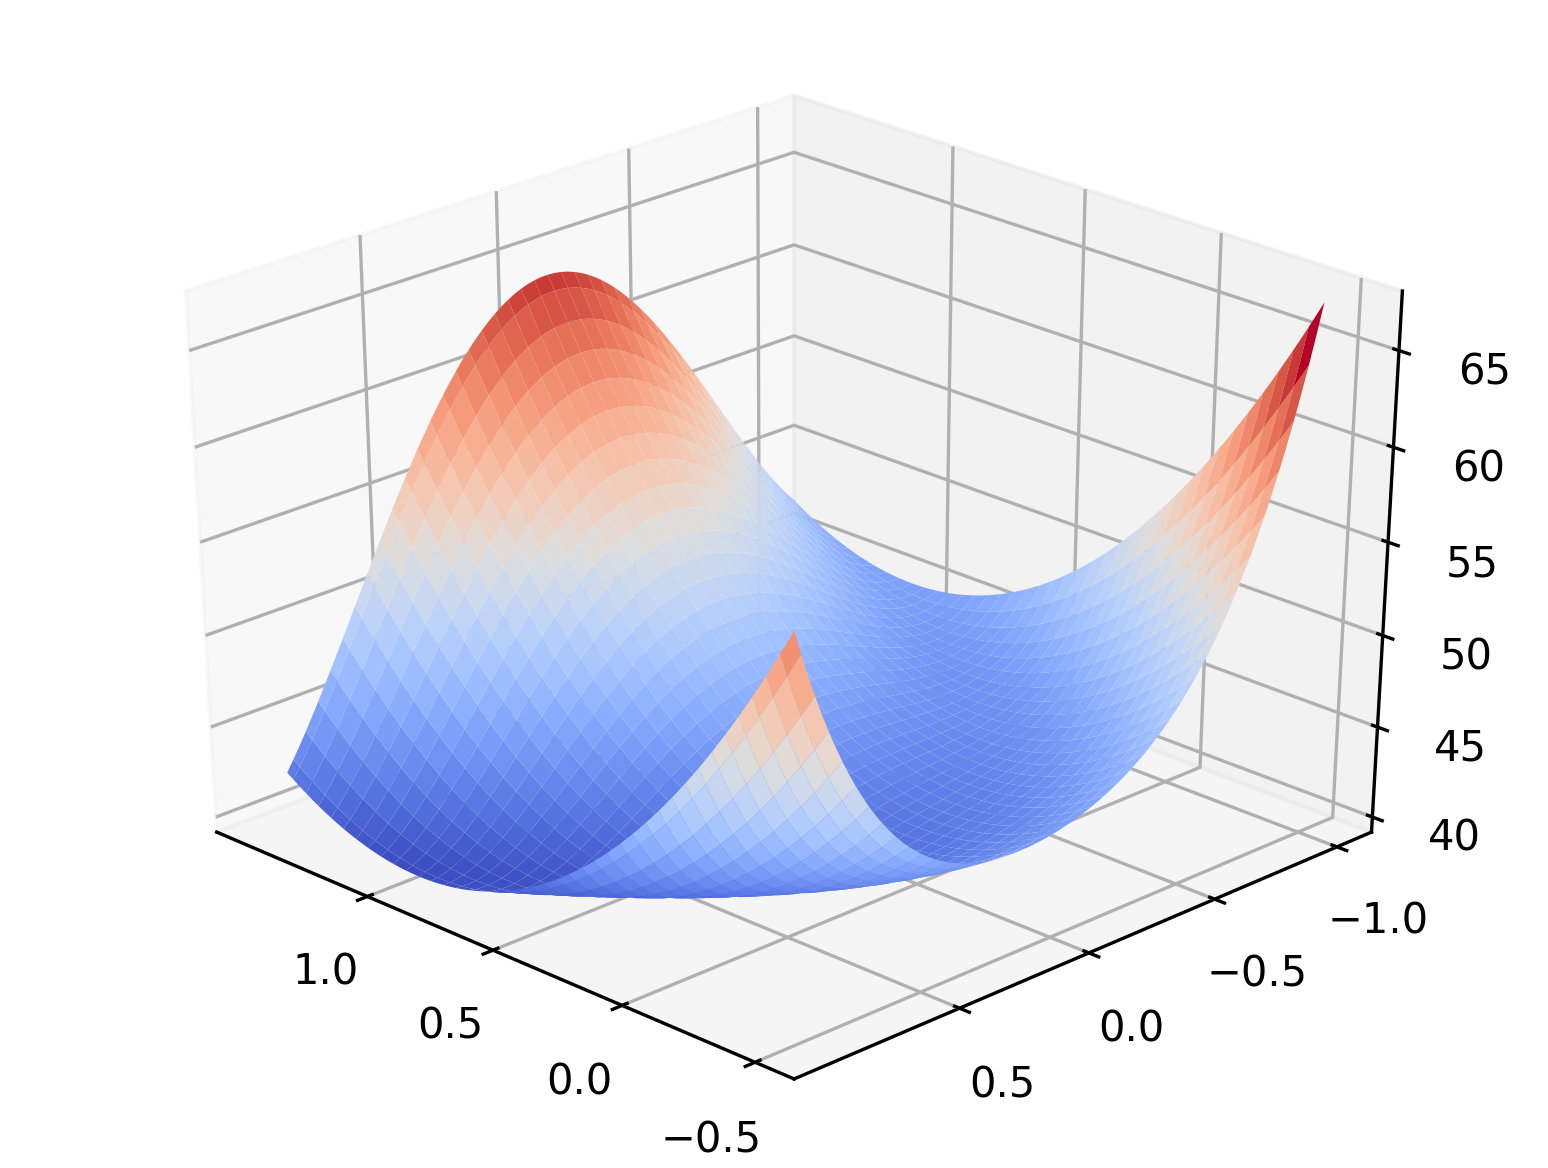
\includegraphics[width=0.48\textwidth]{3d_rosenbrock}} 
%     \subfloat[{$f(x,y) = \frac{\partial}{\partial x} \left[ e^{-\frac{x^2+y^2}{5}} \right]$}]{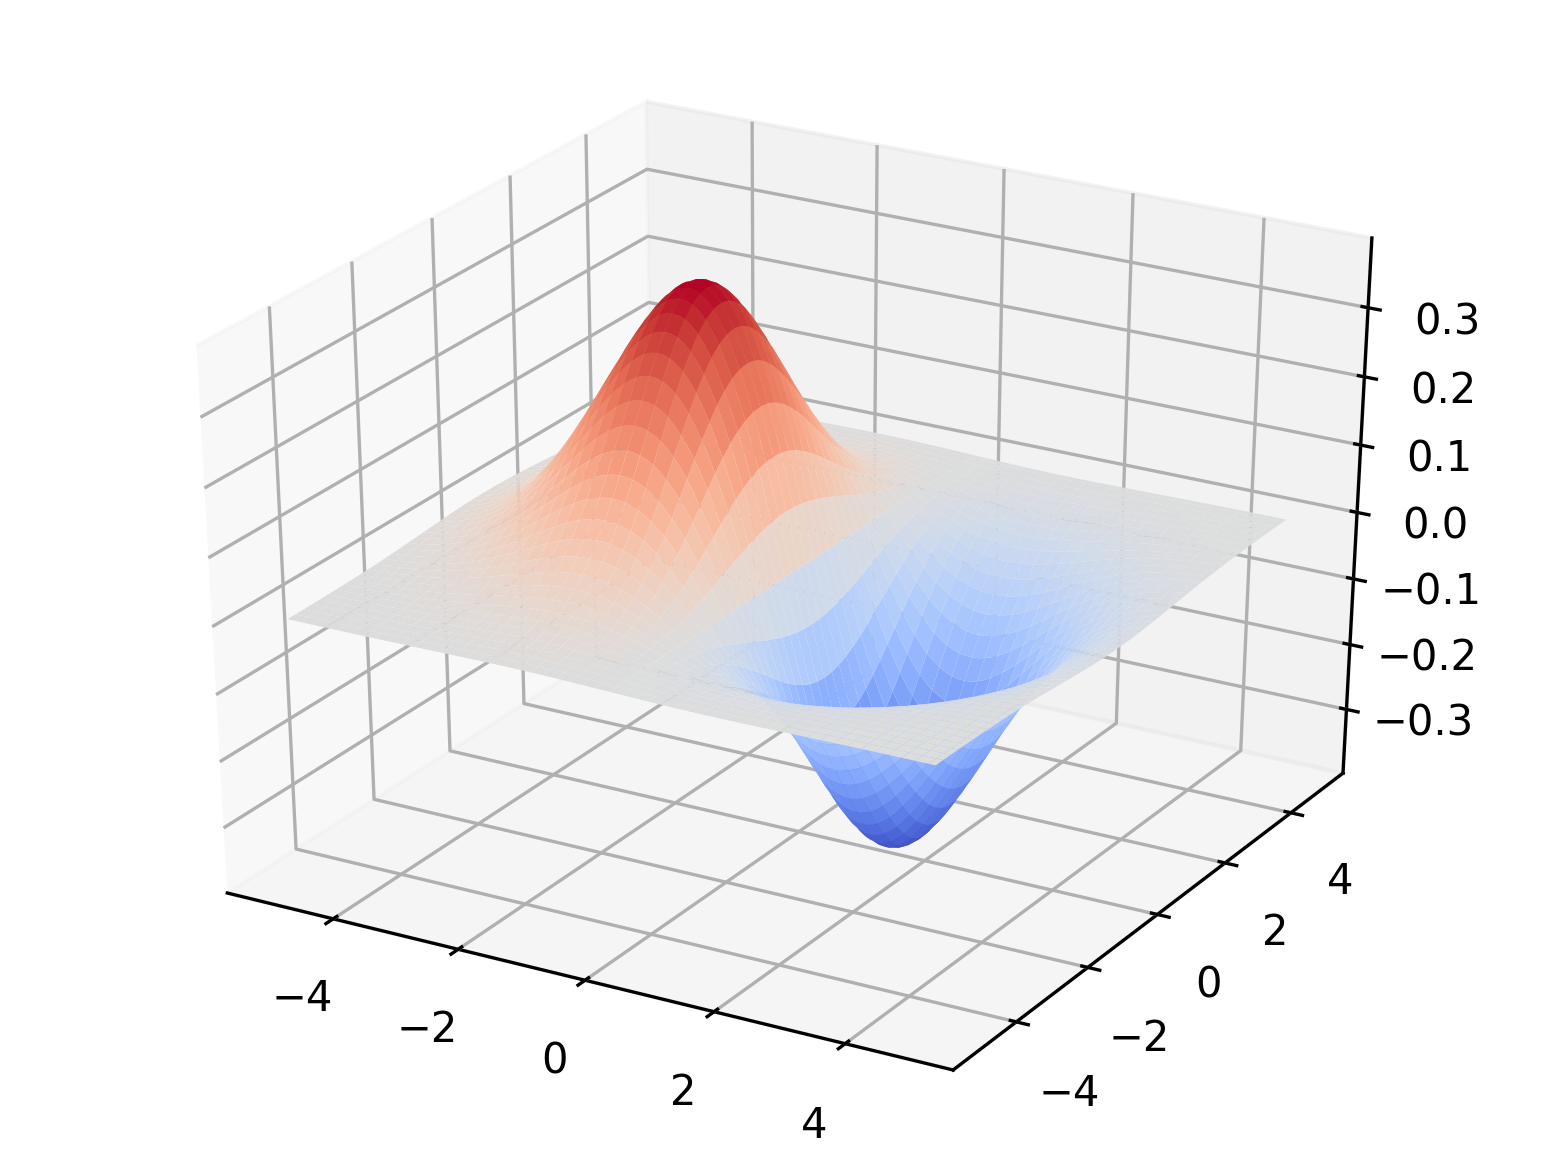
\includegraphics[width=0.48\textwidth]{3d_gauss}}
    
%     \centering
%     \caption{Numerische Optimierungsverfahren ermöglichen es, globale Minima mehrdimensionaler Verlustfunktionen zu finden.}
%     \label{fig:optimierung}
% \end{figure}

\begin{figure}[htbp]
    \captionsetup{justification=centering}

    \centering
    %\subfloat[$f(x,y) = \frac{x^2 - y^2}{5}$]{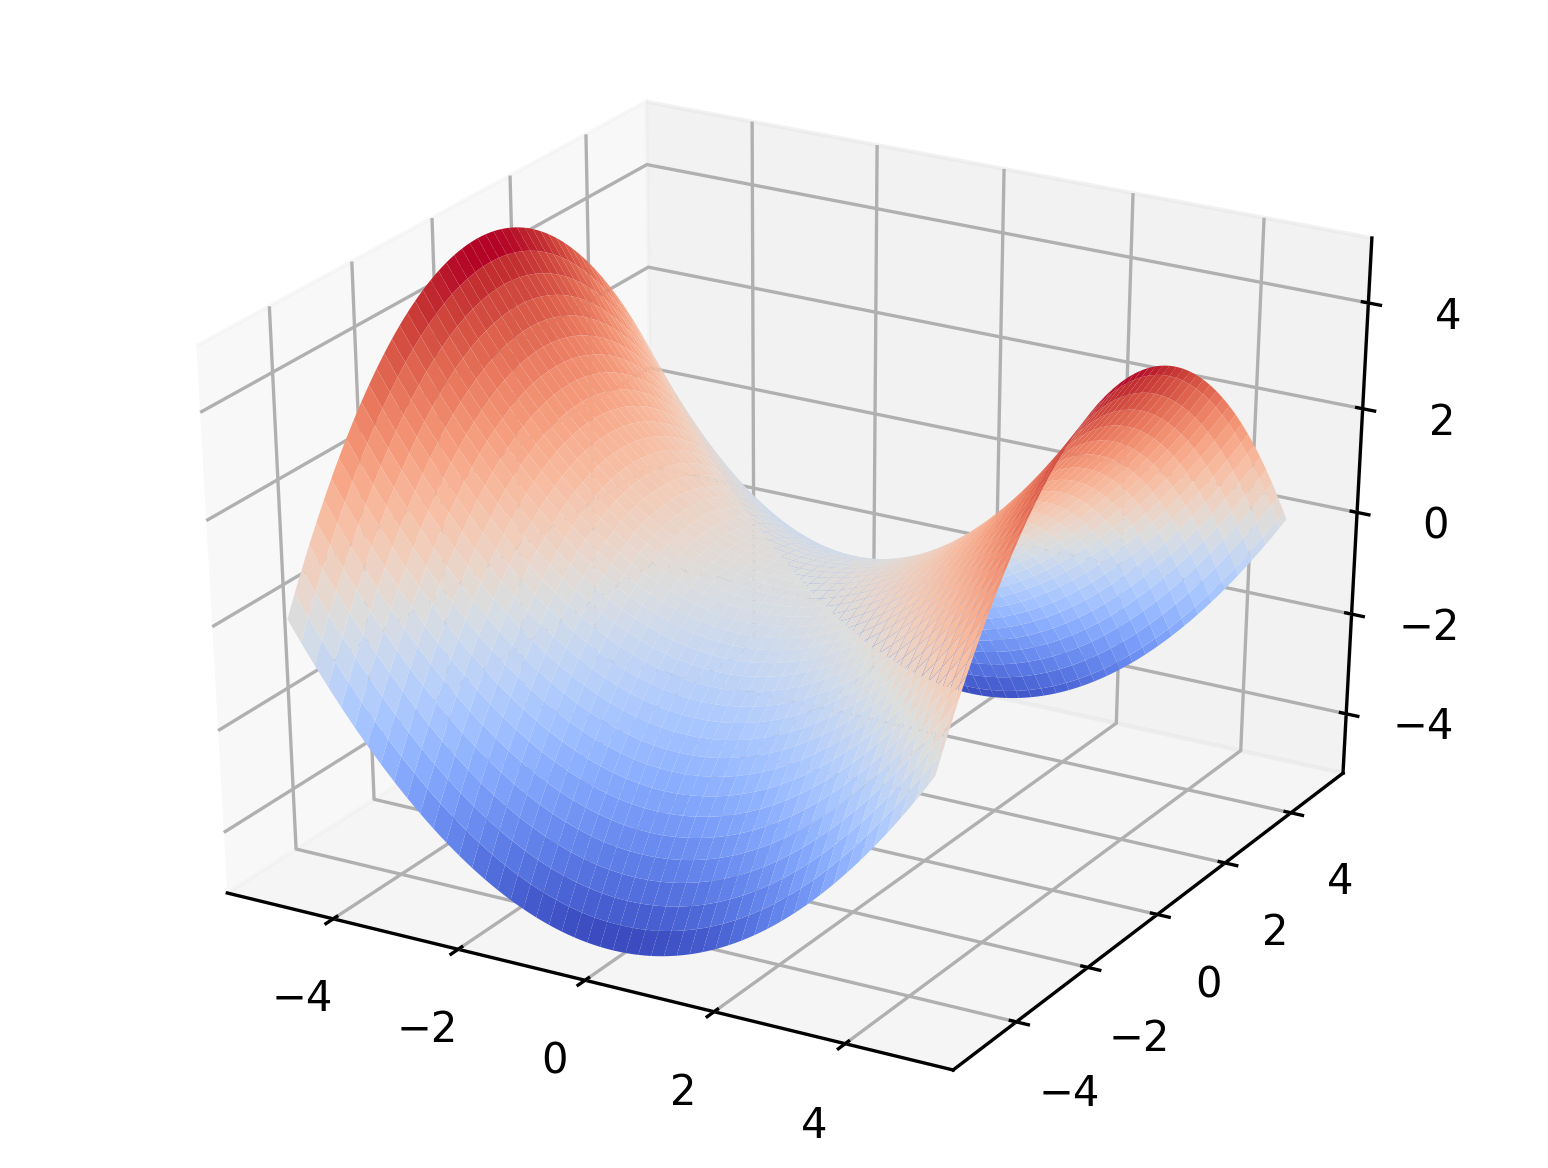
\includegraphics[width=0.48\textwidth]{3d_pringle}} 
    \subfloat[lineare Regression\label{fig:linear:a}]{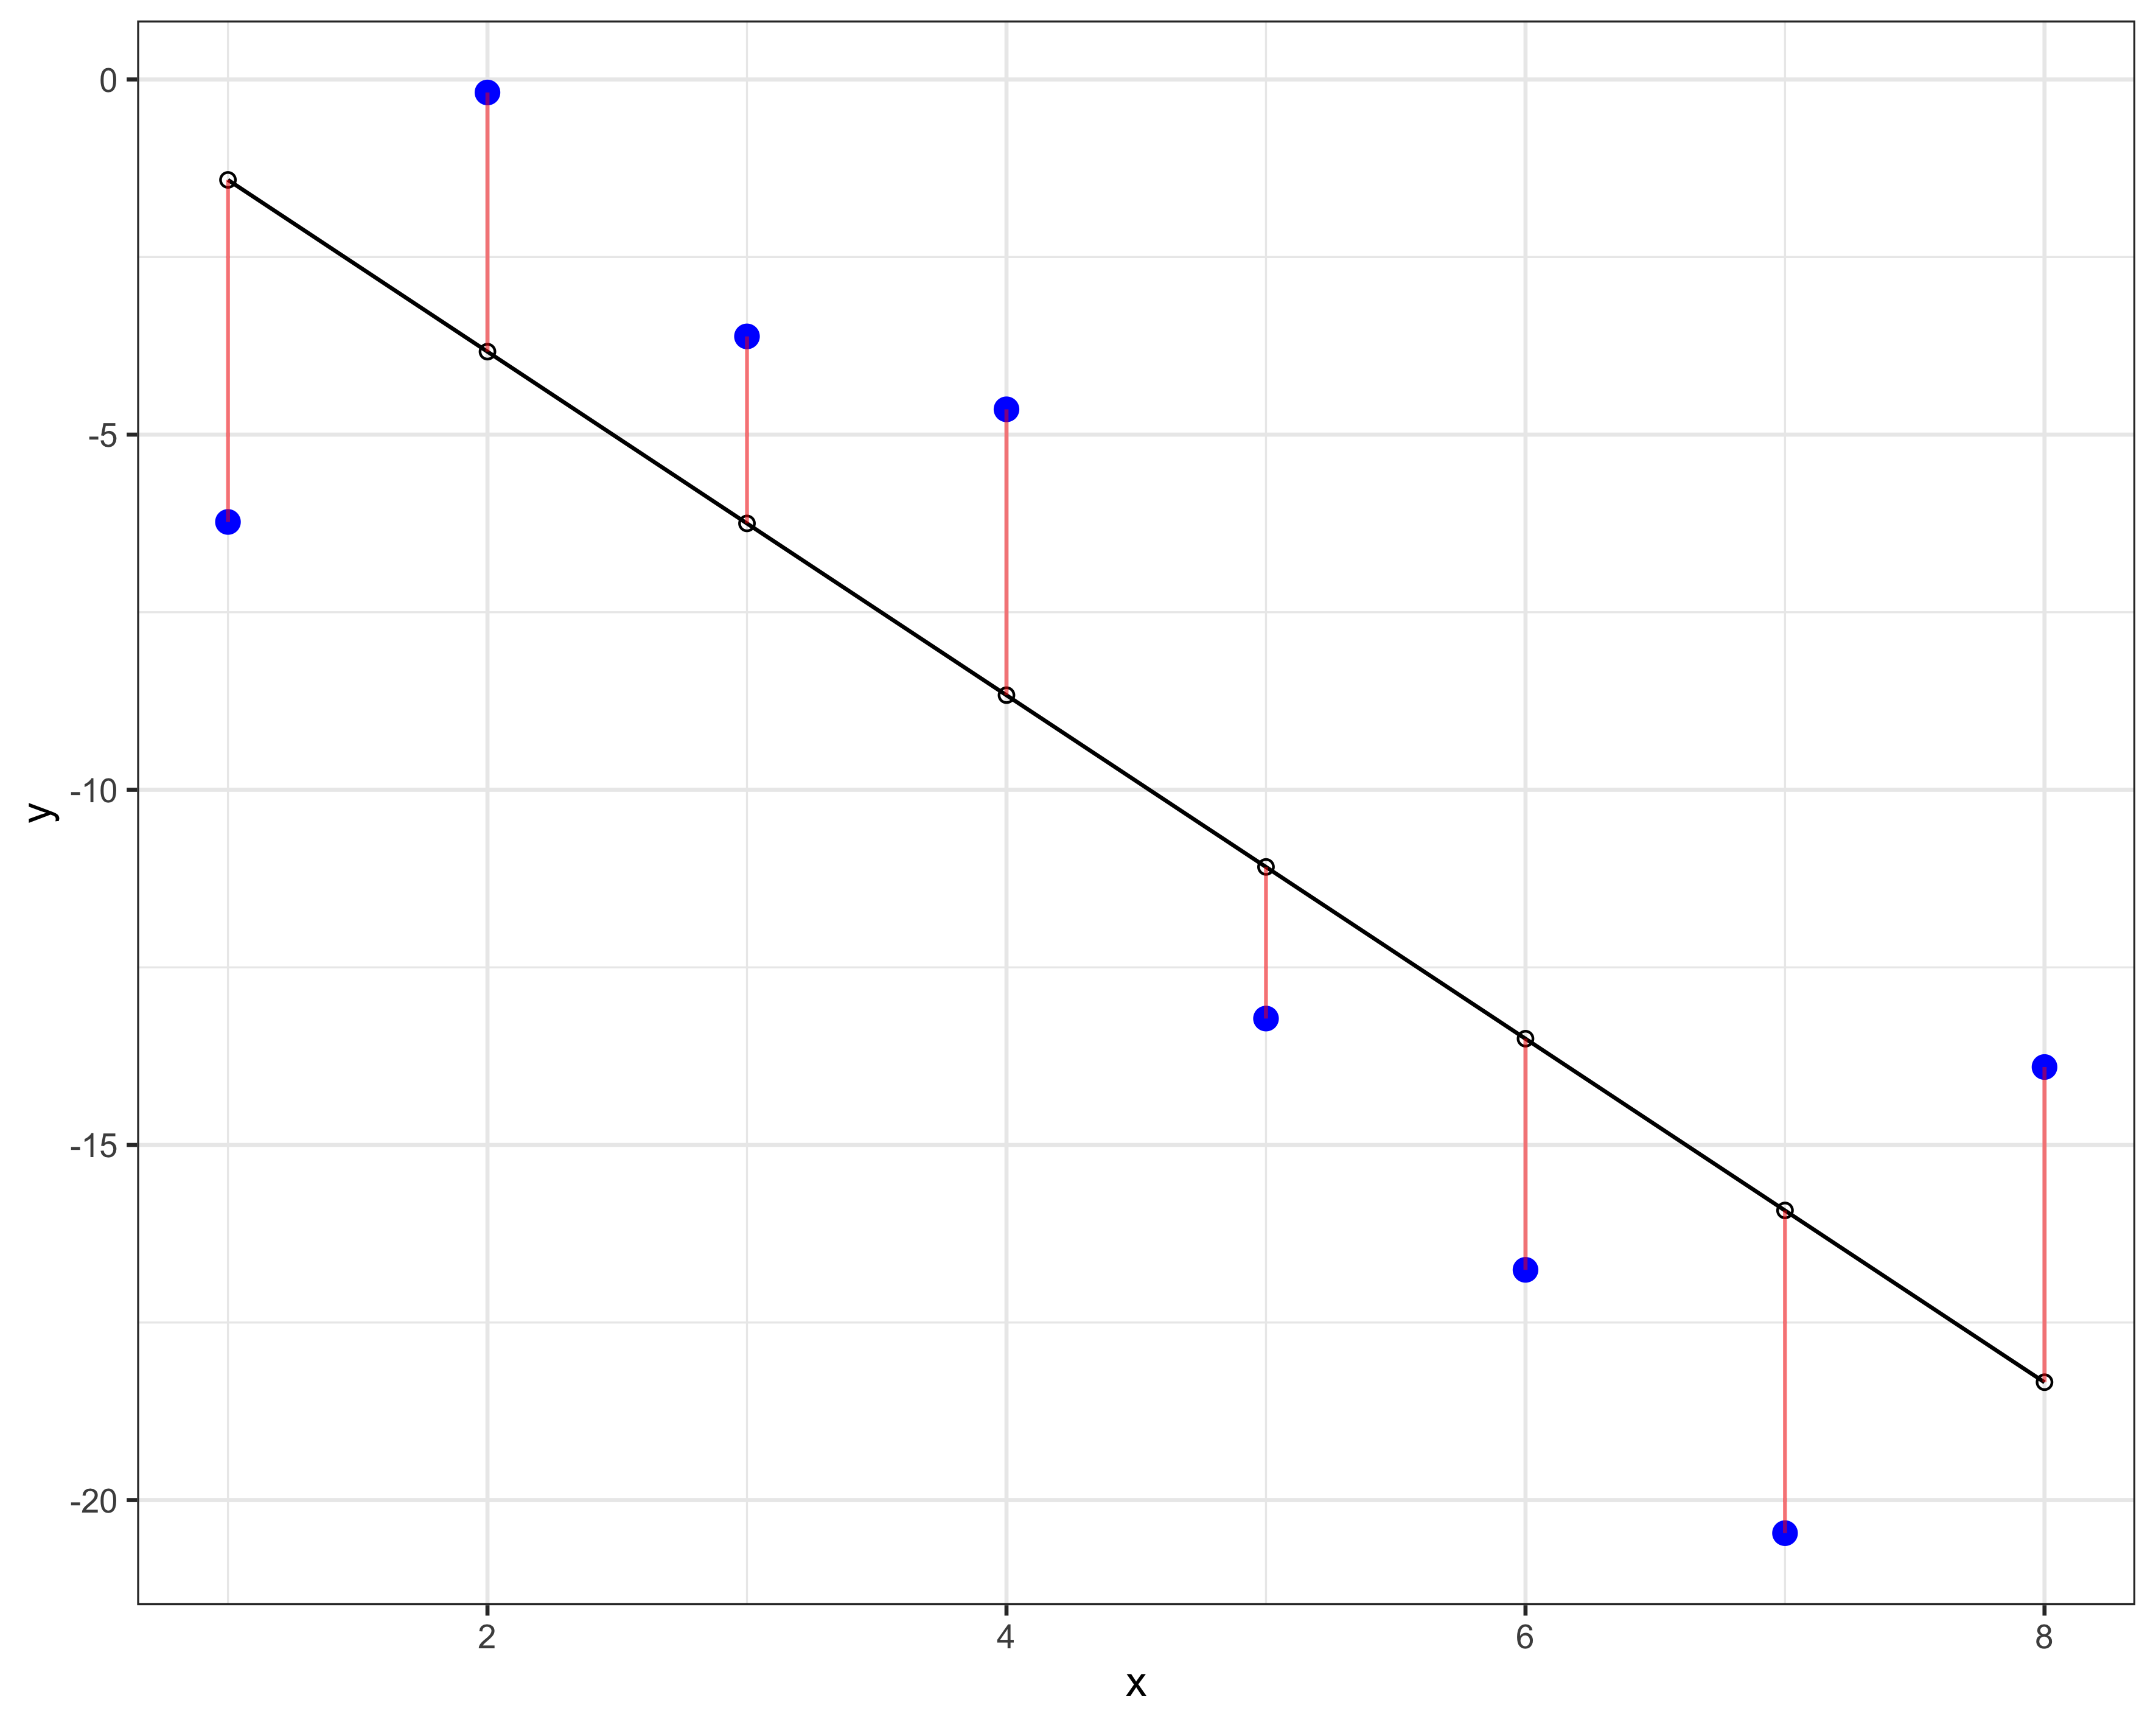
\includegraphics[width=0.48\textwidth]{linear}} 
    \subfloat[Die Verlustfunktion hat ein Minimum, das erreicht wird, wenn m und t optimal gewählt werden.\label{fig:linear:b}]{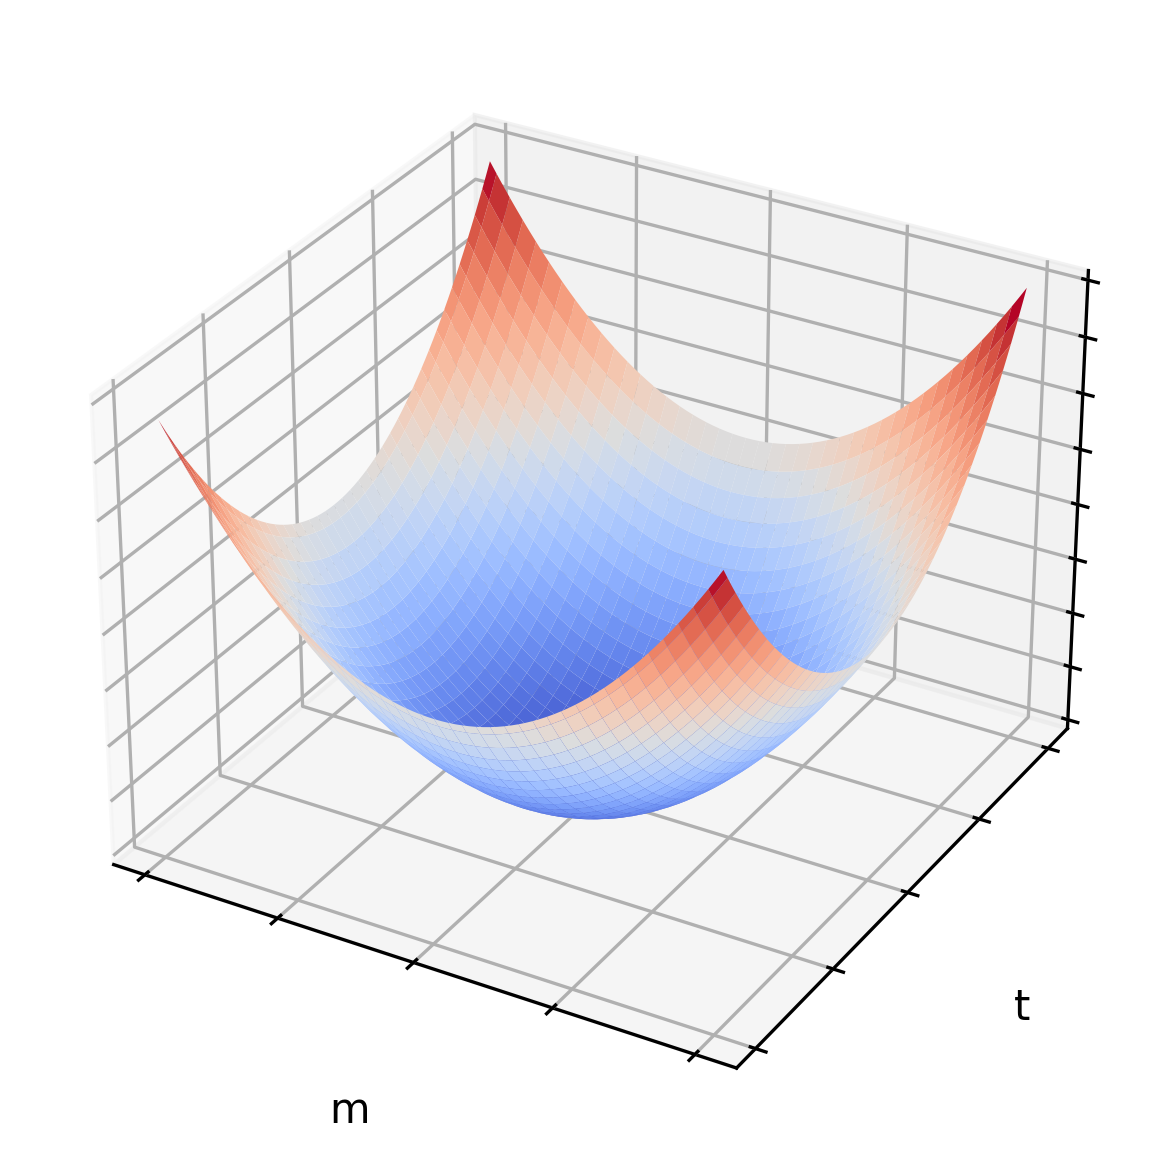
\includegraphics[width=0.48\textwidth]{3d_mt}}
    
    \centering
    \caption{}
    \label{fig:linear}
\end{figure}

\subsection{Überwachtes Lernen}\label{section:supervised_learning}

Algorithmen basierend auf Datensätzen, die sowohl Eingabedaten als auch die dazugehörigen Ausgabedaten enthalten, werden dem überwachten Lernen (\textit{supervised learning}) zugeordnet \citep{russellArtificialIntelligenceModern2020}. Es liegen also Wertepaare vor, die zu jedem Eingabewert auch den gesuchten Ausgabewert enthalten. Im Falle der vorliegenden Arbeit handelt es sich bei den Eingabedaten um Visitentexte und bei den Ausgabedaten um den entsprechen Wert eines bestimmten Scores. 

Bei der Entwicklung eines solchen Modells werden die vorhandenen Datenpaare in zwei disjunkte Teilmengen aufgeteilt: Die Trainingsmenge enthält die Mehrheit (oft 80 - 90 \%) der Wertepaare, während der Rest der Testmenge zugeordnet wird. Diese Aufteilung kann rein zufällig erfolgen, häufig wird allerdings versucht, die Häufigkeitsverteilung der möglichen Ein- und Ausgabewerte in beiden Mengen beizubehalten.

Ein neues Modell wird zunächst anhand der Paare im Trainingsset trainiert. Erst danach wird die Leistung des Modells bewertet, indem seine Vorhersagen auf die Eingabedaten der Testmenge mit den tatsächlichen Werten verglichen werden. Diese Unterteilung ist notwendig, um eine Vorstellung der Leistung des Modells bei unbekannten Daten zu ermöglichen. Erst wenn auch bei Vorhersagen auf der Testmenge eine zufriedenstellende Genauigkeit erreicht wird hat das Modell einen praktischen Nutzen bei der Vorhersage von tatsächlich unbekannten Werten.

\subsection{Overfitting}\label{section:overfitting}
Wird ein Modell zu lange oder auf einem zu kleinen Trainings-Datensatz trainiert, werden unter Umständen in den Eingabedaten Muster erkannt, die nicht vorhanden sind, und zum Beispiel lediglich als Folge statistischer Ungenauigkeiten auftreten. Auf die Trainingsdaten wird so eine sehr hohe prädiktive Genauigkeit erreicht, die sich allerdings nicht auf unbekannte Daten übertragen lässt, da diese die vermeintlichen Muster nicht widerspiegeln. Dieses Problem, im maschinellen Lernen als overfitting (Überanpassung) bezeichnet, wird in Abbildung \ref{fig:overfitting} anhand eines Beispiels verdeutlicht. Hier stellt die orangefarbene Linie ein Modell dar, das zwar sehr gut an die gegebenen Trainingspaare angepasst ist, aber bei neuen Werten deutlich schlechtere Vorhersagen treffen wird als das einfachere Modell (grüne Linie). Das erste Modell wurde in Anbetracht der wenigen Trainingsdaten zu lange trainiert und leidet unter overfitting.

\begin{figure}[htb]
    \centering
    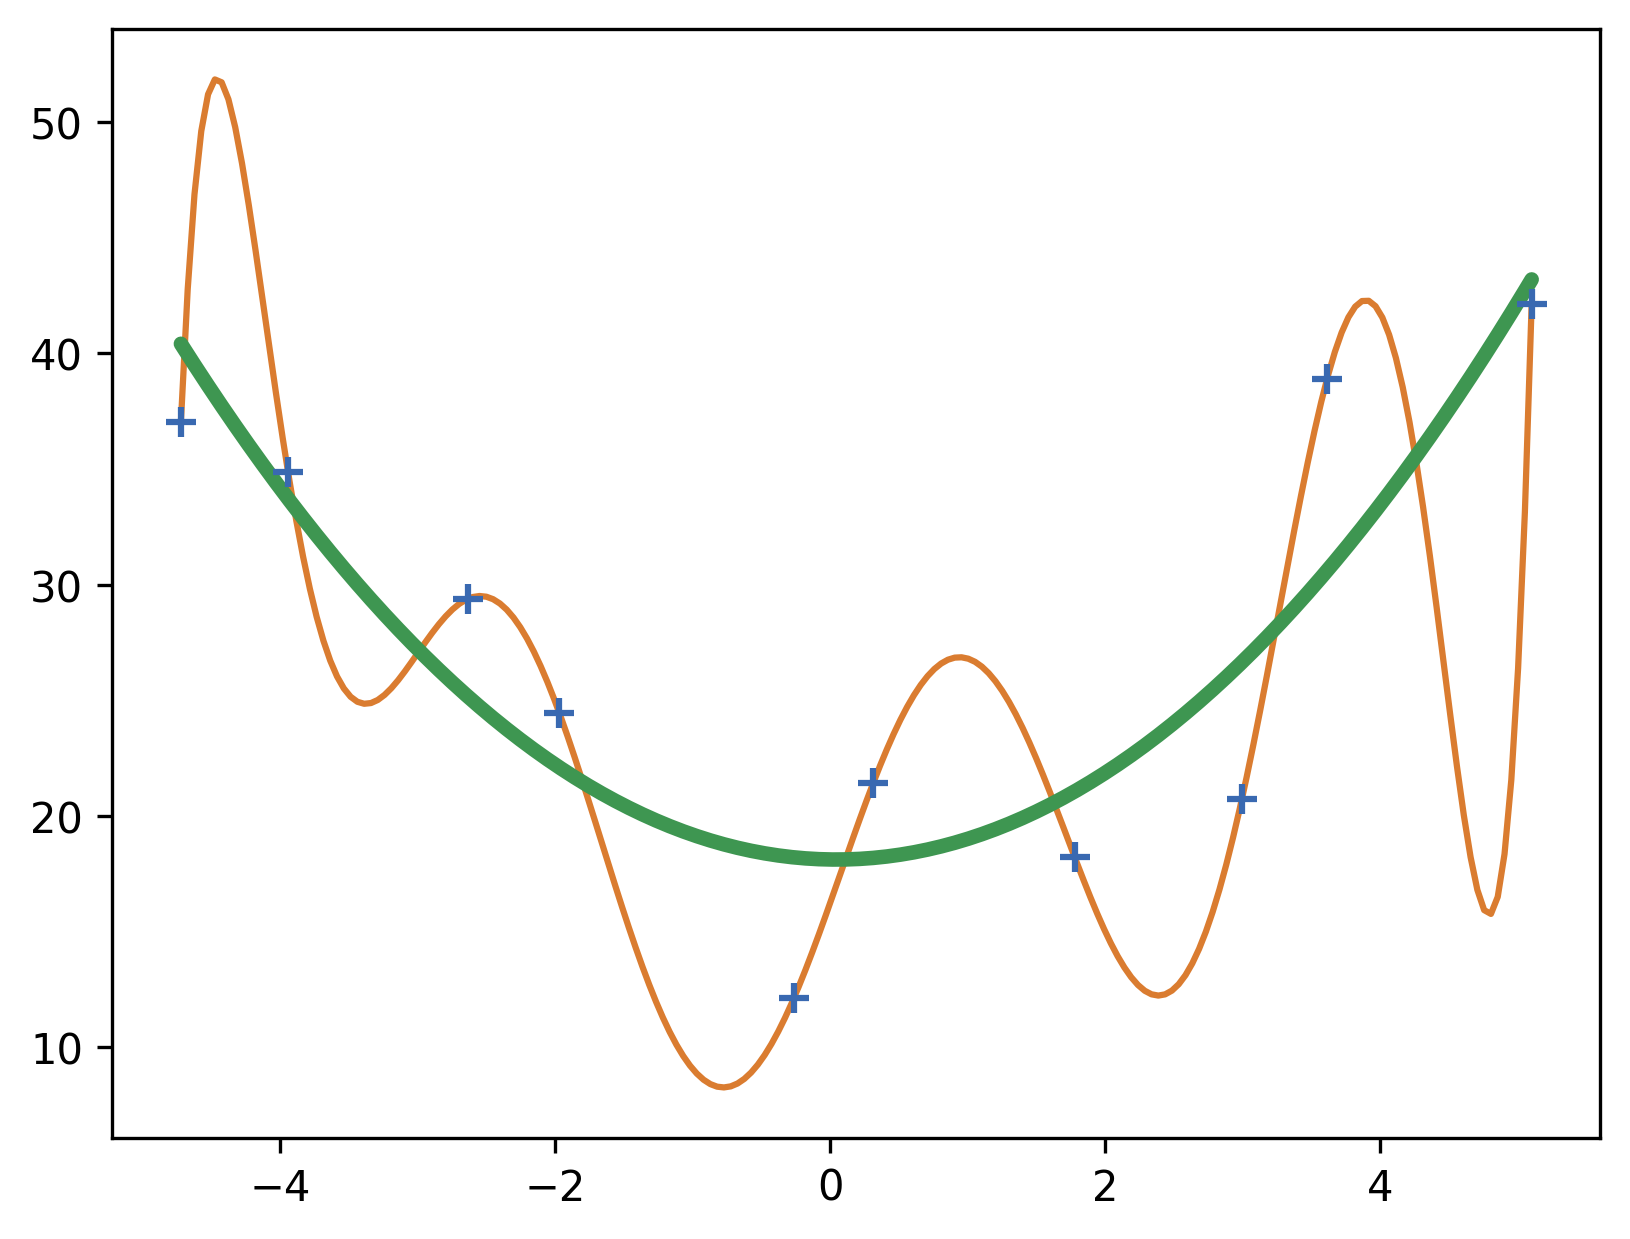
\includegraphics[width=0.6\textwidth]{overfitting}
    \caption{Eine Interpolationspolynom bildet die gegebenen Werte zwar exakt ab, spiegelt aber die tatsächliche Anordnung der Daten schlechter wieder als die grüne Linie.}
    \label{fig:overfitting}
\end{figure} % vielleicht manuell unter den nächsten Absatz verschieben, um Hurenkind auf Seite 8 zu vermeiden

Neben dem überwachten Lernen existieren weitere Arten des maschinellen Lernens, die aber nicht weiter Gegenstand dieser Arbeit sind. Insbesondere das unüberwachte Lernen, bei dem ein Algorithmus versucht, in ungelabelten Datensätzen vorher noch unbekannte Muster zu erkennen \citep{russellArtificialIntelligenceModern2020}, hat hohe Relevanz in anderen Anwendungsfällen des maschinellen Lernens.

\subsection{Regression oder Klassifikation}\label{section:regrvsclf}
Probleme aus dem Bereich des überwachten maschinellen Lernens lassen sich im Allgemeinen weiter in eine von zwei Unterkategorien einordnen: Regression und Klassifikation. Eine Regressionsanalyse verfolgt das Ziel, anhand von einer oder mehrerer unabhängiger Variablen Vorhersagen über eine abhängige Variable zu treffen. Bei der Klassifikation hingegen wird ein gegebener Eingabewert einer oder mehreren Klassen aus einer endlichen Liste möglicher Klassen zugeordnet.\footnote{Typische Anwendungsfälle sind beispielsweise Spam-Filter, die eine E-Mail als "Spam" oder "Nicht Spam" kategorisieren, oder Modelle zur Handschrifterkennung, bei dem jeweils ein handgeschriebenes Zeichen einem von endlich vielen möglichen Buchstaben aus einem gegebenen Alphabet zugeordnet wird.}
Da es sich bei den betrachteten medizinischen Scores um diskrete, ganzzahlige Werte aus einem endlichen Wertebereich handelt, liegt auch hier die Anwendung eines Klassifizierungs-Verfahrens nahe.

Würde man aber die verschiedenen möglichen Werte eines Scores als separate und voneinander unabhängige Klassen betrachten, so ginge die wichtige Information über deren Anordnung verloren. Mit Ausnahme des CAM-ICU\footnote{Dieser fällt entweder positiv oder negativ aus.} handelt es sich bei den im Rahmen dieser Arbeit behandelten Scores stets um eindimensionale, metrische Skalen. Im mathematischen Sinne stellen sie Totalordnungen dar: Sie erfüllen also die Anforderungen der Reflexivität, Antisymmetrie, Transitivität und Totalität. Bezeichne $M$ die Menge aller möglichen Werte eines beliebigen medizinischen Scores. Es gilt dann für alle $a,b,c \in M$:

\begin{equation*}
    \centering
    \begin{aligned}[c]
        a \leq a\\
        a \leq b \land b \leq a \; \Rightarrow \; a=b\\
        a \leq b \land b \leq c \; \Rightarrow \; a \leq c\\
        a \leq b \lor b \leq a
    \end{aligned}
    \qquad
    \begin{aligned}[c]
        \text{(Reflexivität)}\\
        \text{(Antisymmetrie)}\\
        \text{(Transitivität)}\\
        \text{(Totalität)}
    \end{aligned}
\end{equation*}

Entsprechend lassen sich die Werte eines Scores vergleichen und in ein Verhältnis setzen. So ist ein RASS-Wert\footnote{Richmond Agitation-Sedation Scale} von $-4$ (tief sediert) beispielsweise deutlich näher an $-3$ (mäßig sediert) als an $+1$ (unruhig). Bei gängigen Verfahren zur Klassifizierung ginge diese Information verloren, da bei Kenngrößen zur Bewertung solcher Modelle nur betrachtet werden kann, ob ein gegebener Eingabetext genau der richtigen Kategorie (dem richtigen Wert) zugeordnet wurde oder nicht. 

Bei der vorliegenden Arbeit habe ich mich demnach dafür entschieden, die Vergabe von Scores anhand von Eingabetexten als klassisches Regressionsproblem zu betrachten und die Ausgaben der Modelle im Zweifelsfall auf den nächstmöglichen ganzzahligen Wert zu runden. Die Abweichung des vorhergesagten Werts eines Modells von dem nächstmöglichen Wert stellt somit sogar einen rudimentären Ansatz zur Bewertung der Konfidenz einzelner Vorhersagen dar. %siehe: https://stats.stackexchange.com/a/282890

\subsection{Maschinelles Lernen in der Medizin}
Das Vorhandensein großer, digital vorliegender Datensätze stellt eine geeignete Grundlage für ein breites Spektrum an Anwendungen des maschinellen Lernens in der Medizin dar \citep{chenHowDevelopMachine2019}. Ziel dieses Abschnitts ist es, einen exemplarischen, aber keinesfalls erschöpfenden Überblick über einige weitere solcher Anwendungsfälle zu geben.

% Klinikalltag
Im Klinikalltag können Methoden des maschinellen Lernens Ärzten bei der Auswertung von Befunden sowie beim Erkennen klinisch relevanter Muster in Bilddaten unterstützen \citep{shahArtificialIntelligenceMachine2019}. Auch bei der Diagnostik wird ML angewendet, beispielsweise zur computergestützten Auskultation \citep{reedHeartSoundAnalysis2004}. In der Intensivmedizin werden mittels ML vorliegende Datensätze ausgewertet, unter anderem um Komplikationen vorherzusagen, Mortalitätsraten zu bestimmen und prognostische Modelle zu verbessern \citep{shillanUseMachineLearning2019, krishnanSupervisedLearningApproach2018}.

% Arzneimittelforschung
Außerhalb der Klinik findet maschinelles Lernen auch im Bereich der Arzneimittelforschung Anwendung. Hier werden derartige Modelle unter anderem dazu eingesetzt, neue Targetproteine für bestimmte Wirkstoffe zu identifizieren, effizientere Wirkstoffkombinationen zu entwickeln und ein besseres Verständnis komplexer Krankheitsmechanismen zu erlangen \citep{vamathevanApplicationsMachineLearning2019}.

% Virologie
In der Virologie wird maschinelles Lernen unter anderem dazu angewandt, die Ausbreitung von Infektionskrankheiten zu modellieren \citep{9121027}. Weiterhin werden Risikofaktoren für eine Infektion ermittelt und Prädiktoren für die Mortalität bereits infizierter Personen identifiziert. Derartige Informationen ermöglichen es, Handlungsempfehlungen für behandelnde Ärzte und Pflegekräfte \citep{colubriMachineLearningPrognosticModels2019} sowie politische Entscheidungsträger \citep{satuMachineLearningBasedApproaches2020} zu formulieren.

% Explainable AI/CDSS
Zuletzt sei die in der Medizin besonders relevante Problematik der Explainable AI erwähnt. Ohne spezielle Maßnahmen ähneln Modelle des maschinellen Lernens, insbesondere künstliche neuronale Netze, einer Art Black Box. Sie sind zwar oft in der Lage, beeindruckende Leistungen in ihrer Domäne zu erzielen, ihre genaue Wirkungsweise ist aber oft selbst für die Entwickler nicht vollumfänglich verständlich. Beispielsweise sollen sogenannte clinical decision support systems\footnote{klinische Entscheidungsunterstützungssysteme} Ärzten bei der Entscheidungsfindung im Klinikalltag assistieren, indem große Datenmengen automatisch analysiert und aufbereitet werden. Insbesondere bei Entscheidungen, die einen hohen Einfluss auf das Patientenoutcome haben, stellt sich die Frage, in welchem Maße den oft schwer nachvollziehbaren Empfehlungen einer Maschine vertraut werden sollte.